\begin{figure}[h!]
\begin{center}
\caption{Educational Attainment by Region: 1990-2010}
\label{fig:EducRegion}
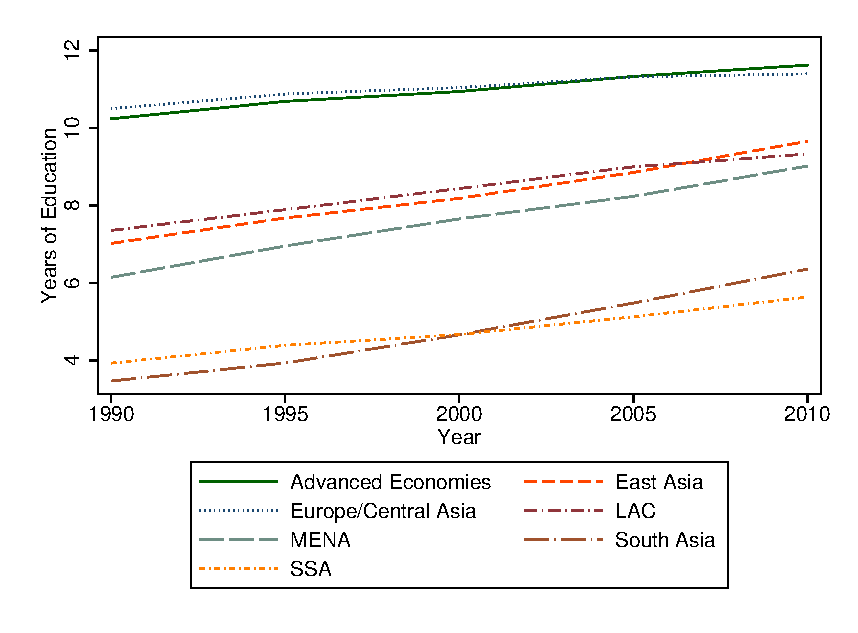
\includegraphics[scale=0.9]{\MMRfolder/Results/graphs/trends/SchoolingRegion.eps} 
\end{center}
\end{figure}

\begin{figure}[h!]
\begin{center}
\caption{Maternal Mortality Ratio by Region: 1990-2010}
\label{fig:MMRRegion}
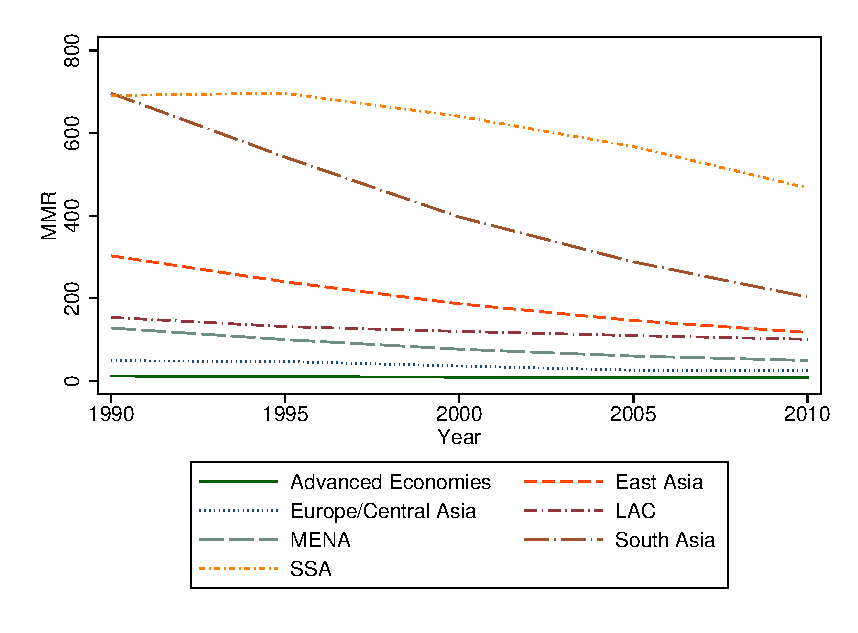
\includegraphics[scale=0.9]{\MMRfolder/Results/graphs/trends/MMRRegion.eps} 
\end{center}
\end{figure}

\begin{figure}[h!]
\begin{center}
\caption{Maternal Mortality and Education: Functional Form}
\label{fig:educmmr}
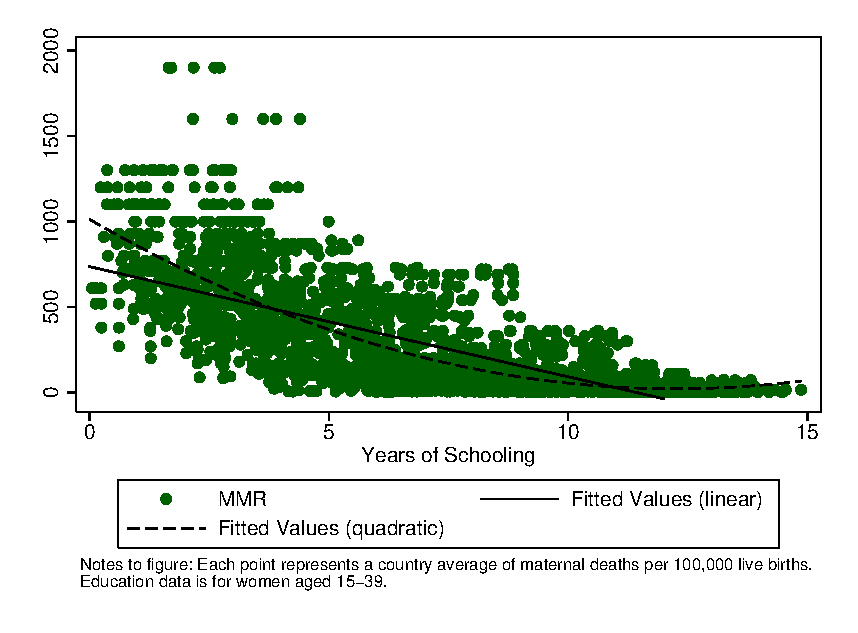
\includegraphics[scale=0.9]{\MMRfolder/Results/graphs/trends/Schooling_MMR_F.eps} 
\end{center}
\end{figure}

\begin{figure}[h!]
\begin{center}
\caption{Between and Within Country Correlations: Education and MMR}
\label{fig:arrows}
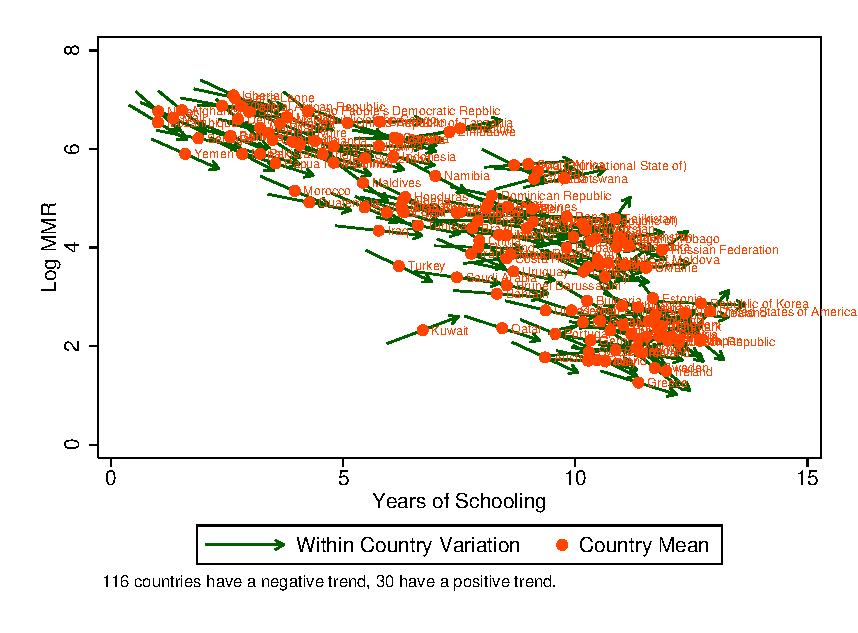
\includegraphics[scale=0.9]{\MMRfolder/Results/graphs/countries.eps} 
\end{center}
\end{figure}


\begin{landscape}
\begin{figure}[h!]
\begin{center}
\caption{Maternal Mortality Ratio by Country}
\label{fig:MMRGlobal}
\includegraphics[scale=0.9]{\MMRfolder/Results_aug2013/Graphs/MMR_2010.eps} 
\end{center}
\end{figure}
\end{landscape}


\begin{subfigures}
\begin{figure}[h!]
\begin{center}
\caption{Educational Attainment by Year -- Nigeria}
\label{fig:Nigeriaeduc}
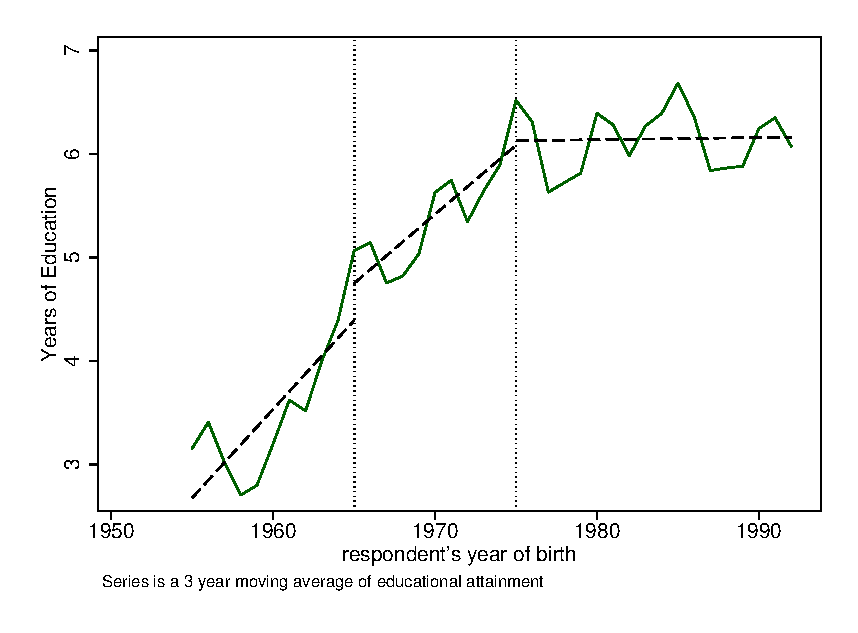
\includegraphics[scale=0.85]{\MMRfolder/Results/graphs/Nigeria_educ.eps} 
\end{center}
\end{figure}

\begin{figure}[h!]
\begin{center}
\caption{Maternal Mortality by Year -- Nigeria}
\label{fig:Nigeriammr}
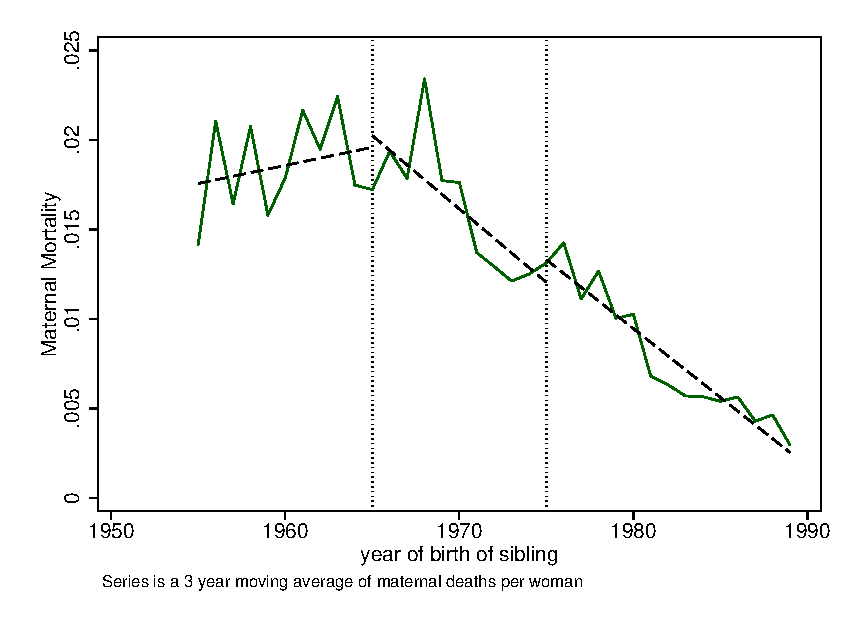
\includegraphics[scale=0.85]{\MMRfolder/Results/graphs/Nigeria_mmr.eps} 
\end{center}
\floatfoot{Note to figures \ref{fig:Nigeriaeduc}-\ref{fig:Nigeriammr}: 3 year moving
averages are displayed for maternal mortality and education.  The first vertical
dotted line represents the end of the control group, and the second vertical dotted
line represents the beginning of fully treated cohorts. Cohorts in between are
partially treated.  Further details in the body of the text, and table 
\ref{MMRtab:EducExp}.}
\end{figure}
\end{subfigures}

\clearpage

\begin{subfigures}
\begin{figure}[h!]
\begin{center}
\caption{Educational Attainment by Year -- Kenya}
\label{fig:Kenyaaeduc}
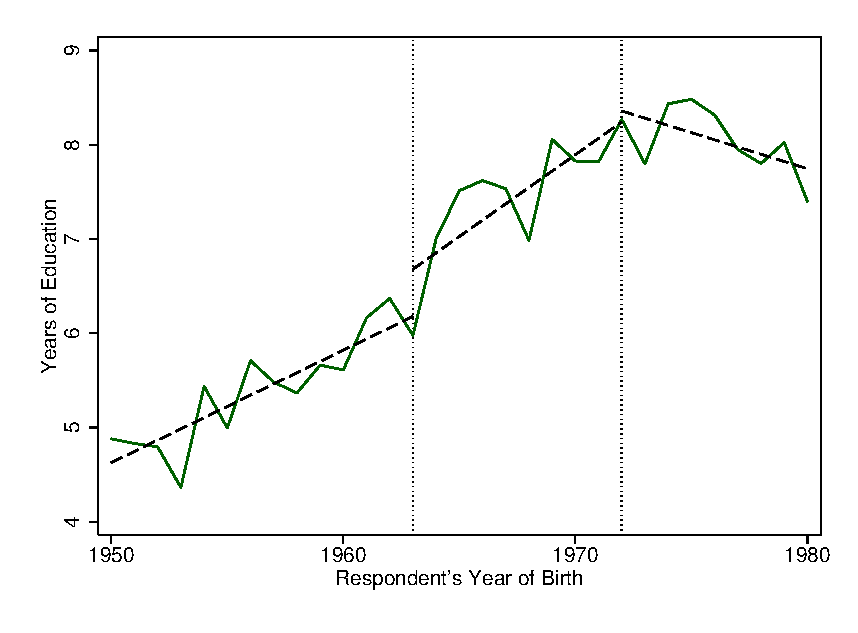
\includegraphics[scale=0.85]{\MMRfolder/Results/graphs/Kenya_educ.eps} 
\end{center}
\end{figure}

\begin{figure}[h!]
\begin{center}
\caption{Maternal Mortality by Year -- Kenya}
\label{fig:Kenyammr}
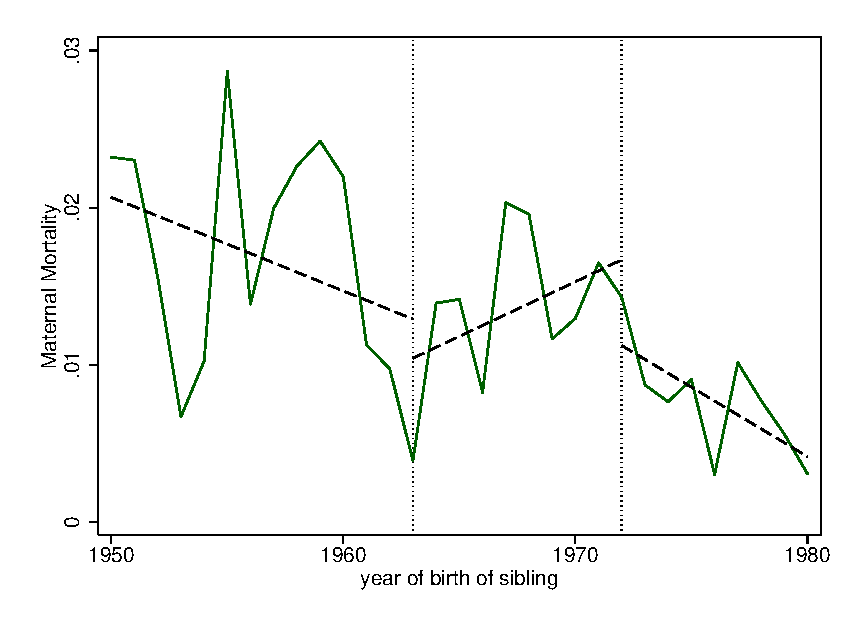
\includegraphics[scale=0.85]{\MMRfolder/Results/graphs/Kenya_mmr.eps} 
\end{center}
\floatfoot{Note to figures \ref{fig:Kenyaaeduc}-\ref{fig:Kenyammr}: The first 
vertical dotted line represents the end of the control group, and the second 
vertical dotted line represents the beginning of fully treated cohorts. Cohorts 
in between are partially treated.  Further details are provided in the body of 
the text, and in table \ref{MMRtab:EducExp}.}
\end{figure}
\end{subfigures}

\clearpage

\begin{subfigures}
\begin{figure}[h!]
\begin{center}
\caption{Educational Attainment by Year -- Zimbabwe}
\label{fig:Zimbabweeduc}
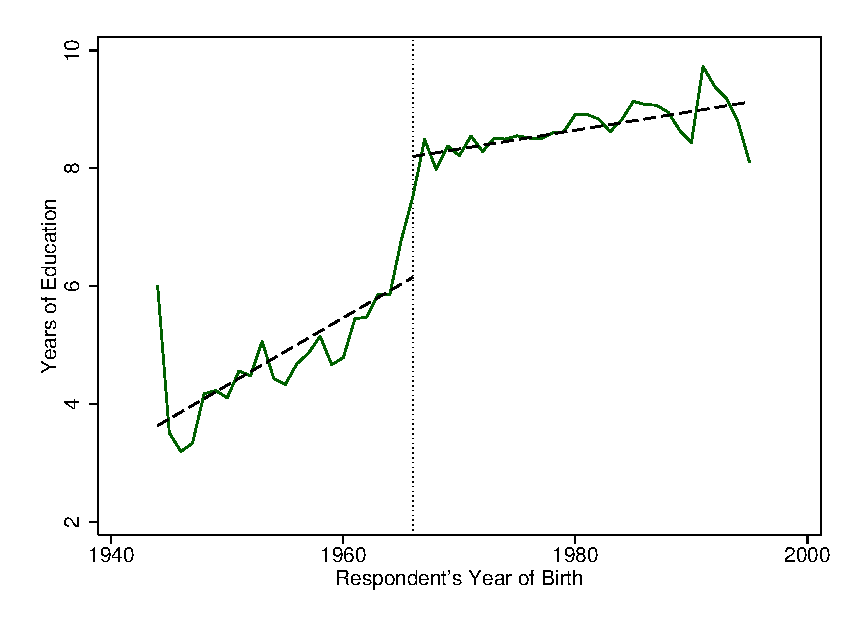
\includegraphics[scale=0.85]{\MMRfolder/Results/graphs/Zimbabwe_educ.eps} 
\end{center}
\end{figure}

\begin{figure}[h!]
\begin{center}
\caption{Maternal Mortality by Year -- Zimbabwe}
\label{fig:Zimbabwemmr}
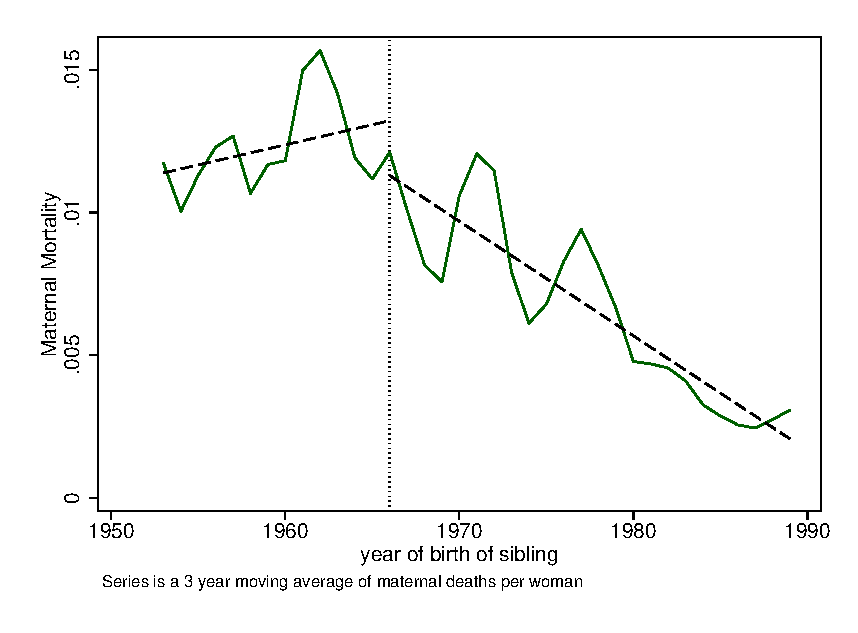
\includegraphics[scale=0.85]{\MMRfolder/Results/graphs/Zimbabwe_mmr.eps} 
\end{center}
\floatfoot{Note to figures \ref{fig:Zimbabweeduc}-\ref{fig:Zimbabwemmr}: 
Treatment was a one year expansion in schooling, differentially affecting
\emph{only} the 1965/1966 cohorts.  All cohorts to the left of the vertical
dotted line (1966 and after) are considered treated, and all cohorts to the 
right of the line (1965 and before) are not treated. Further details are 
provided in the body of the text, and in table \ref{MMRtab:EducExp}.}
\end{figure}
\end{subfigures}

\clearpage
